% tikzpic.tex
\documentclass[crop]{standalone}% 'crop' is the default for v1.0, before it was 'preview'
\usepackage{testpackage}
\setromanfont{Fira Sans}
\setmainfont{Fira Sans}
\everymath\expandafter{\the\everymath\rm}
\everydisplay\expandafter{\the\everydisplay\rm}
%\usetikzlibrary{...}% tikz package already loaded by 'tikz' option
\usepackage{tikz,pgfplots}
\usepackage{array}
 
\begin{document}
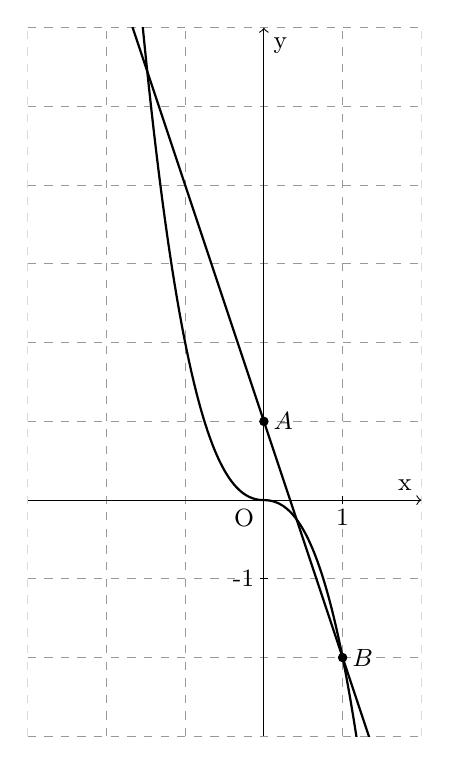
\begin{tikzpicture}
\clip (-3,-3) rectangle (2,6);\draw[color=black!40,dashed] (-3,-3) grid (2,6);
\draw[->](-3,0)--(2,0) node[above left]{\small x};\draw[->](0,-3)--(0,6)node[below right]{\small y};;
\draw[thick] plot[domain=-3:3,samples=200,variable=\x,] (\x,-\x^3-\x^2);
\draw[thick] plot[domain=-3:3,samples=10,variable=\x,] (\x,-3*\x+1);
\node[below left] at (0,0){\small O};
\node[circle,draw=black,fill,inner sep=0pt,minimum size=3pt] at (0,1){};\node[right] at (0,1){\small$A$};
\node[circle,draw=black,fill,inner sep=0pt,minimum size=3pt] at (1,-2){};\node[right] at (1,-2){\small$B$};
\draw(1,-0.05)--(1,0.05);\node[below] at (1,0){\small 1};\node[left] at (0,-1){\small -1};
\draw(-0.05,-1)--(0.05,-1);
\end{tikzpicture}
\end{document} 